\documentclass[letterpaper,10pt]{extarticle}
\usepackage[utf8]{inputenc}
\usepackage[T1]{fontenc}
\usepackage{graphicx}
\usepackage[x11names]{xcolor}
\usepackage{tikz}
\usetikzlibrary{circuits.ee.IEC}
\usepackage[os=win]{menukeys}

\usepackage{amsmath,amssymb,textcomp}
\everymath{\displaystyle}

\usepackage{physics}

\usepackage{times}
\renewcommand\familydefault{\sfdefault}
\usepackage{tgheros}
\usepackage{droidmono}

\usepackage{enumitem}
\usepackage[explicit]{titlesec}

\usepackage{multicol}
\setlength{\columnseprule}{0pt}
\setlength{\columnsep}{15.0pt}

\usepackage{geometry}
\geometry{left=10mm,right=10mm,top=10mm,bottom=15mm,showframe=false}

% custom title
\makeatletter
\renewcommand*{\maketitle}{%
\noindent
\begin{minipage}{0.82\textwidth}

\begin{tikzpicture}
\node[rectangle,rounded corners=6pt,inner sep=6pt,fill=SteelBlue1,text width=.95\textwidth] {\color{black}\huge \@title};
\end{tikzpicture}
\end{minipage}
\hfill
\begin{minipage}{0.17\textwidth}
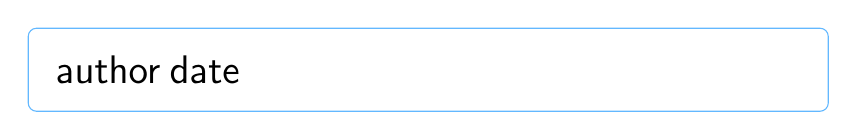
\begin{tikzpicture}
\node[rectangle,rounded corners=3pt,inner sep=10pt,draw=SteelBlue1,text width= 0.78\textwidth] {\raggedleft \Large \@author\ \@date};
\end{tikzpicture}
\end{minipage}
%\bigskip%\bigskip
}%
\makeatother

% custom section
\newcommand*\sectionlabel{}
\titleformat{\section}
  {\gdef\sectionlabel{}
   \normalfont\sffamily\Large\bfseries\scshape}
  {\gdef\sectionlabel{\thesection\ }}{0pt}
  {
\noindent
\begin{tikzpicture}
\node[rectangle,rounded corners=3pt,inner sep=4pt,fill=DodgerBlue4,text width= 0.95\columnwidth] {\color{white}\sectionlabel#1};
\end{tikzpicture}
  }
\titlespacing*{\section}{0pt}{.5pt}{0.5pt}

% custom subsection
\newcommand*\subsectionlabel{}
\titleformat{\subsection}{\normalfont\sffamily\bfseries\scshape}{\subsectionlabel}{0pt}{
\noindent
\begin{tikzpicture}
\node[rectangle,rounded corners=4pt,inner sep=3pt,fill=DodgerBlue3,text width= 0.95\columnwidth] {\color{white}\subsectionlabel#1};
\end{tikzpicture}
}
\titlespacing*{\subsection}{0pt}{.5pt}{.5pt}

% custom subsubsection
\newcommand*\subsubsectionlabel{}
\titleformat{\subsubsection}{\normalfont\sffamily\small\bfseries\scshape}{\subsubsectionlabel}{0pt}{
\noindent
\begin{tikzpicture}
\node[rectangle,rounded corners=3pt,inner sep=3pt,fill=blue!50!yellow,text width= 0.95\columnwidth] {\color{white}\subsubsectionlabel#1};
\end{tikzpicture}
}
\titlespacing*{\subsubsection}{0pt}{.5pt}{.5pt}


\title{GPA220 : Analyse des circuits électriques}
\author{INTRA}
\date{A2018}

%\linespread{1.3}

\begin{document}
\maketitle

\begin{multicols*}{2}

\setlength{\belowdisplayskip}{2.5pt}
\setlength{\belowdisplayshortskip}{2.5pt}
\setlength{\abovedisplayskip}{2.5pt}
\setlength{\abovedisplayshortskip}{2.5pt}

\section{Notion de base}
\vspace{-1.75\baselineskip}
\subsection{Puissance électrique}
\begin{equation*}
    P = VI = R I^2 = \frac{V^2}{R} \qty[W] \qq{}|\; P_{\mathrm{fournie}} < 0 < P_{\mathrm{consommee}}
\end{equation*}

% \subsection{Loi d'Ohm et Convention des signes}
\begin{multicols*}{2}
\subsection{Loi d'Ohm}
\centering
\begin{equation*}
    V = RI \Leftrightarrow R=\frac{V}{I}
\end{equation*}

\subsection{Convention passive}
%\vspace{-2\baselineskip}
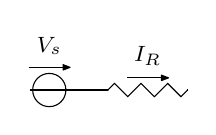
\begin{tikzpicture}[circuit ee IEC,
                    every info/.style={font=\footnotesize},
                    small circuit symbols,
                    set resistor graphic=var resistor IEC graphic]
  \draw (0,0) to [voltage source={near start, direction info={info=$V_s$}}] (1,0)
              to [resistor={direction info={info=$I_R$}}] (2,0);
\end{tikzpicture}
\end{multicols*}

\subsection{Résistances en série}
\begin{equation*}
    R_{\mathit{eq}}=R_1 + R_2 + \dots + R_N
\end{equation*}
\begin{itemize}[nosep]
    \item Différences de potentiel s'additionnent \( \Delta V = \Delta V_1 +\Delta V_2 \)
    \item Courants identiques \( I= I_1 = I_2\)
\end{itemize}

\subsection{Résistances en parallèle}
\begin{equation*}
    R_{\mathit{eq}}=\qty(\frac{1}{R_1}+\frac{1}{R_2}+\dots +\frac{1}{R_N})^{-1}
\end{equation*}
\begin{itemize}[nosep]
    \item Différences de potentiel identique \( \Delta V = \Delta V_1 =\Delta V_2 \)
    \item Courants s'additionnent \( I = I_1 + I_2\)
\end{itemize}

\subsection{Transformation $\Delta-Y$}
\centering
%  trim={<left> <lower> <right> <upper>}
\includegraphics[trim={2in 7.5in 2in 1.25in}, clip=true,page=15,height=1.25in]{fig/note2.pdf}
\begin{align*}
    R_1 &= \frac{R_b R_c}{R_a + R_b + R_c}\\
    R_2 &= \frac{R_a R_c}{R_a + R_b + R_c}\\
    R_3 &= \frac{R_a R_b}{R_a + R_b + R_c}
\end{align*}
\raggedright

\section{Analyse de circuit}
%\vspace{-2\baselineskip}
\subsection{Kirchhoff}
%\vspace{-1\baselineskip}
\begin{multicols*}{2}
\subsubsection{Loi des noeuds}
%\vspace{-1\baselineskip}
\begin{equation*}
    \sum I = 0
\end{equation*}
    
\subsubsection{Loi des mailles}
%\vspace{-1\baselineskip}
\begin{equation*}
    \sum \Delta V =0
\end{equation*}
\end{multicols*}

\subsubsection{Étapes de résolution d'un circuit}
\begin{enumerate}%[nosep]
    \item Assigner un courant dans chaque branche : Direction arbitraire, si le courant est négatif, alors le courant circule en sens contraire.
    \item Écrire les équations de tous les noeuds sauf un. $(n-1)$
    \item Écrire les équations de diverses mailles jusqu'à l'obtention de $X$ équations pour $X$ inconnues; chaque branche doit être parcourue aux moins une fois.
\end{enumerate}
% \subsubsection{Sens du courant}


\section{Techniques d’analyse de circuits}
% \vspace{-.5\baselineskip}
\subsection{Transformation de source}
% \vspace{-1\baselineskip}
Seulement possible s'il n'y a pas de source dépendante dans le circuit.
\begin{multicols*}{2} 
\centering
%  trim={<left> <lower> <right> <upper>}
\includegraphics[trim={1.75in 8.375in 1.75in 1in}, clip=true,page=2,height=.85in]{fig/equiv.pdf}

\begin{equation*}
    I_s = \frac{V_s}{R}
\end{equation*}
\end{multicols*}
\vspace{-1\baselineskip}

% \vspace{-1\baselineskip}
\subsubsection{Cas particulier}
\begin{itemize}[nosep]
    \item Résistance en $//$ avec $V_s$ peut être ignorée.
    \item Résistance en série avec $i_s$ peut être ignorée.
\end{itemize}


\subsection{Équivalents Thévenin et Norton}
\begin{equation*}
    R_{Th}=\frac{V_{Th}}{I_{cc}}
\end{equation*}
Cas particulier, si le circuit n'a pas de source dépendante. 
\begin{itemize}[nosep]
    \item Source de tension $=$ court-circuit
    \item Source de courant $=$ circuit ouvert
\end{itemize}
\subsubsection{Étapes de résolution}
\begin{enumerate}
    \item Calculer la tension de Thévenin $V_{Th}$
    \item Calculer le courant de court-circuit $I_{cc}$
    \item Calculer la résistance de Thévenin $R_{Th}$
    \item Re-dessiner le circuit équivalent Thévenin
\end{enumerate}

\subsubsection{Équivalent Norton}
On obtient l'équivalent Norton en faisant une transformation de source de l'équivalent Thévenin.


\subsection{Transfert maximal de puissance}
La puissance consommée par la charge $R_L$ est: 
%\vspace{-.5\baselineskip}
\begin{equation*}
    P = VI = R_L I^2 = R_L \qty(\frac{V_{Th}}{R_{Th}+R_L})^2
\end{equation*}
Résistance $R_L$ pour obtenir un transfert de puissance maximal
%\vspace{-1\baselineskip}
\begin{equation*}
    R_L = R_{Th}
\end{equation*}
La puissance transférée à la charge:
%\vspace{-.375\baselineskip}
\begin{equation*}
    P_{max} = \frac{V^2_{Th}}{4R_L}
\end{equation*}
% %\vspace{-1\baselineskip}
% Please add the following required packages to your document preamble:
% \usepackage{graphicx}
% \begin{table}[h]
% \caption{Inductance}
\section{Circuits RL et RC}
\subsection{Inductance}
% \resizebox{.45\textwidth}{!}{%
\centering
\begin{tabular}{lll}
Valeur & Formule & Unitée \\\hline\rule{0pt}{15pt}
Tension      & \(v=L\frac{di}{dt} \) & V \\[5pt]
Courant      & \(i(t)=\frac{1}{L}\int_{t_0}^{t} v \;d \tau + i(t_0) \) & A \\[5pt]
Puissance    & \(p=Li\frac{di}{dt} \) & W \\[5pt]
Énergie      & \(w=\frac{1}{2}Li^2\) & J \\[5pt]\hline\rule{0pt}{15pt}
Const. de temps & \(\tau = \frac{L}{R} \)& s\\[5pt]\hline\rule{0pt}{15pt}
En série     & \(L_{eq} = L_1 + \dots + L_n\) &   \\
En parallèle & \(L_{eq} = \qty(\frac{1}{L_1} + \dots + \frac{1}{L_n})^{-1} \) & 
\end{tabular}%
% }

\subsection{Condensateur}
\centering
\begin{tabular}{lll}
Valeur & Formule & Unitée \\\hline\rule{0pt}{15pt}
Tension      & \(v=\frac{1}{C}\int_{0}^{t} i \;d \tau + v(0)  \) & V \\[10pt]
Courant      & \(i(t)=C\frac{dv}{dt}\) & A \\[5pt]
Puissance    & \(p(t)=vi=Cv\frac{dv}{dt} \) & W \\[5pt]
Énergie      & \(w=\frac{1}{2}Cv^2\) & J \\[5pt]\hline\rule{0pt}{10pt}
Const. de temps & \(\tau = RC\) & \\\hline\rule{0pt}{5pt}
En série     & \(C_{eq} = \qty(\frac{1}{C_1} + \dots + \frac{1}{C_n})^{-1} \) &   \\[10pt]
En parallèle & \(C_{eq} = C_1 + \dots + C_n\) &  
\end{tabular}%

\subsection{Analyse de circuits}
\resizebox{.475\textwidth}{!}{%
\begin{tabular}{ll|l}
&	Réponse naturelle & Réponse forcée (échelon) \\\hline
& Dissipation de l'énergie. & Ajout d'une source d'énergie. \\
RL & \( i(t) = i_0 e^{-\frac{t}{\tau}} \) & \( i(t) = \frac{V_s}{R} + \qty(I_0 - \frac{V_s}{R}) e^{-\frac{R}{L}t} \) \\
RC & \( v(t) = V_0 e^{-\frac{t}{RC}} \) & \( v(t) = I_s R + \qty(V_0 - I_s R) e^{-\frac{t}{RC}} \)
\end{tabular}
}

\subsubsection{Conditions initiales}
\begin{tabular}{c|c}
    RL & RC \\
    $i_L = I_s$ & $i_C = 0$\\
    $v_L = 0$ & $v_C = V_s$
\end{tabular}


\section{Préfixes Système International}
\begin{tabular}{lll}
Facteur    & Nom   & Symbol \\\hline\\[-1em]
$10^{6}$   & mega  & M      \\
$10^3$     & kilo  & k      \\
$10^{-3}$  & milli & m      \\
$10^{-6}$  & micro & $\mu$  \\
$10^{-9}$  & nano  & n      \\
$10^{-12}$ & pico  & p     
\end{tabular}

\end{multicols*}

\end{document}
